\documentclass{article}%
\usepackage[T1]{fontenc}%
\usepackage[utf8]{inputenc}%
\usepackage{lmodern}%
\usepackage{textcomp}%
\usepackage{lastpage}%
\usepackage{authblk}%
\usepackage{graphicx}%
%
\title{Localization of the Intracellular Activity Domain of Pasteurella multocida Toxin to the N Terminus}%
\author{Denise Fowler}%
\affil{School of Dentistry, Chung Shan Medical University, Taichung 40201, Taiwan}%
\date{01{-}01{-}2014}%
%
\begin{document}%
\normalsize%
\maketitle%
\section{Abstract}%
\label{sec:Abstract}%
Please enable Javascript to watch this video\newline%
Global trends show that tumor heterogeneity is driving the advance of targeted drugs in human health. The label using Genentech and Roche to use PRIX for the treatment of HER2 positive and HER3 positive breast cancer, shows that each patient with (chemotherapy){-}positive or with metastatic disease will receive a distinct PATIENTS targeted drug tailored to specifically target tumor heterogeneity.\newline%
PATIENTS with extremely large tumor populations are particularly resistant to therapy, and tumors with small to marginal tumor heterogeneity offer greater degrees of heterogeneity that act to drive the drugs against specific targets on the tumor.\newline%
There is a possibility that cancer cells that have very large tumor populations will have immunogenic characteristics similar to those that have small or marginal tumor heterogeneity. For example, if a large tumor cell is found outside of the normal white blood cell population, that tumor cell might attract the immune system to attack it. This type of pathogenic means of immunogenic characteristics has been widely reported in other human cancers such as lung, brain, and blood cancers.\newline%
Genentech and Roche determined in animal models what their patients respond to therapy using PRIX. They did this by selecting and defining cancer cells which were extremely large tumor populations, (i) predefined in their genetic material (i.e. PLA 61, GL 2, GbH41, etc.) and (ii) had a RECIST (Positive, Incomplete, or Recipient function) with a higher than normal response. They identified these abnormally large tumors by adding them to the tumor exposure assay. Next, they combined PRIX with immunologic profiling to identify the specific tumor cells that respond to treatment with the drug.\newline%
Researchers found that in breast cancer patients with larger, genetic breast cancer, drugs administered to them will kill these abnormal tumor cells more efficiently than the ones that belong to the healthy breast population. Within the cancer patients, those with the largest tumor populations have more cell death that occurs after treatment with PRIX.\newline%
Both Genentech and Roche have defined patisinib as a very high{-}risk treatment, and they are developing two additional once{-}daily/weekly regimens designed to improve outcomes and reduce overall treatment costs.

%
\subsection{Image Analysis}%
\label{subsec:ImageAnalysis}%


\begin{figure}[h!]%
\centering%
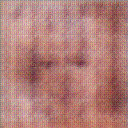
\includegraphics[width=150px]{500_fake_images/samples_5_498.png}%
\caption{A Close Up Of A Number Of Different Colored Tooth Brushes}%
\end{figure}

%
\end{document}